% !TeX root=../main.tex
\chapter{دانش پیش‌زمینه}
%\thispagestyle{empty} 
\section{مقدمه} 
در این فصل مفاهیم مورد نیاز و استفاده در این پروژه مورد بررسی قرار می‌گیرند.
این فصل، محل شرح کامل روش تحقیق است و بسته به نوع روش تحقیق و با نظر استاد راهنما می‌تواند «مواد و روش‌ها%
\LTRfootnote{Materials and Methods}»
نیز نام بگیرد. این فصل حدود ۱۵ صفحه است.

\section{شبکه‌های مبتنی بر نرم‌افزار}

% \section{NetKAT}
نت‌کت، یک زبان برای توصیف شبکه‌های مبتنی بر نرم‌افزار است
\cite{netkat}.
این زبان با وجود سینتکس ساده‌ای که دارد، بر اساس
KAT
\cite{kat}
بنا شده و به همین دلیل یک سیستم معادلاتی کامل و صحیح دارد.
این سیستم معادلاتی کمک می‌کند تا با استفاده از روش‌های جبری و اثبات تساوی برنامه‌های توصیف شده در این زبان، در مورد آن‌ها استدلال کرد.

\subsection{سینتکس NetKAT}
در نت‌کت هر بسته به عنوان یک نگاشت از یک مجموعه از فیلد‌های
$f_1,f_2,...,f_n$
به اعداد طبیعی با تعداد ارقام ثابت در نظر گرفته می‌شود.
آی‌پی‌های مبدا و مقصد، نوع بسته، پورت‌های مبدا و مقصد مثال‌هایی از این فیلد‌ها هستند.
برای اینکه امکان استدلال در مورد مسیر‌های طی شده توسط یک بسته‌ در شبکه وجود داشته باشد،از مفهومی به نام تاریخچه‌ی بسته استفاده می‌شود.
هر تاریخچه‌ی بسته‌، یک دنباله از بسته‌ها است که بسته نخست دنباله، به عنوان بسته‌ی فعلی در نظر گرفته می‌شود.
سینتکس نت‌کت به صورت زیر تعریف می‌شود:
\begin{align*}
    a,b ::= & 1 | 0 | f = n | a + b | a \cdot b | \neg a  \\
    p,q ::= & a | f \la n | p + q | p \cdot q | p^* | dup
\end{align*}
به صورت شهودی
عبارت های ۱ و ۰ به ترتیب به معنای عبور دادن و رها کردن بدون شرط بسته هستند.
عبارت
$f=n$
در صورتی بسته را عبور می‌دهد که مقدار فیلد
f
آن برابر با
n
باشد.
عبارت
$f \la n$
مقدار n
را به فیلد f
بسته اختصاص می‌دهد.
به صورت دقیق، معنای هر عبارت با استفاده از معادلات زیر تعریف می‌شود:
\begin{align*}
    \sem{p}             & H \in \mathcal{P}({H})                \\
    \sem{1} h           & \teq \s{h}                            \\
    \sem{0} h           & \teq \s{}                             \\
    \sem{f=n}(pk::h)    & \teq \begin{cases}
                                   \s{pk::h} & \text{ if } pk.f = n \\
                                   \s{}      & \text{ otherwise }
                               \end{cases} \\
    \sem{\neq a}        & \teq \s{h} \setminus (\s{a}h)         \\
    \s{f \la n} (pk::h) & \teq \s{pk[f:=n]::h}                  \\
    \sem{p+q}h          & \teq \sem{p}h \cup \sem{q}h           \\
    \sem{p\cdot q} h    & \teq (\sem{p} \bullet \sem{q}) h      \\
    \sem{p^*}h          & \teq \bigcup_{i \in \mathbb{N}}F^i h  \\
    F^0 h               & \teq \s{h}                            \\
    F^{i+1} h           & \teq (\sem{p} \bullet F^i) h          \\
    (f \bullet g) x     & \teq \bigcup\s{g(y)|y \in f(x)}       \\
    \sem{dup} (pk::h)   & \teq \s{pk::(pk::h)}
\end{align*}
نت‌کت علاوه بر اصول موضوعه‌ی
KAT
اصول‌ موضوعه‌ی زیر را هم شامل می‌شود تا دستگاه معادلاتی کامل داشته باشد:
\begin{align}
    f \la n \cdot f' \la n' & \equiv f' \la n' \cdot f \la n,
    \text{ if } f \neq f' \label{mod-mod-comm}
    \\
    f \la n \cdot f' = n'   & \equiv f' = n' \cdot f \la n,
    \text{ if } f \neq f' \label{mod-filter-comm}                            \\
    dup \cdot f = n         & \equiv f = n \cdot dup \label{dup-filter-comm} \\
    f \la n \cdot f = n     & \equiv f \la n \label{mod-filter}              \\
    f = n \cdot f \la n     & \equiv f = n \label{filter-mod}                \\
    f \la n \cdot f \la n'  & \equiv f \la n' \label{mod-mod}                \\
    f = n \cdot f = n'      & \equiv 0, \text{ if } n \neq n' \label{contra} \\
    \Sigma_{i} f = i        & \equiv 1 \label{match-all}
\end{align}
اصل‌های
\ref{mod-mod-comm},\ref{mod-filter-comm},\ref{dup-filter-comm}
خواص جابه‌جایی عملیات‌ها را بیان می‌کنند.
اصل
\ref{mod-filter}
بیان می‌کند که اختصاص مقدار
n
به یک فیلد و سپس این فیلد با همین مقدار معادل با عملیات اختصاص به تنهایی است.
مشابه همین اصل برای یک فیلتر و سپس یک اختصاص هم در اصل
\ref{filter-mod}
مشخص شده.
اصل
\ref{mod-mod}
بیان می‌کند که در دنباله‌ای از اختصاص مقادیر به یک فیلد مشخص، تنها آخرین اختصاص تاثیر دارد.
در اصل
\ref{contra}
مشخص شده است که مقدار یک فیلد نمی‌تواند دو مقدار متفاوت داشته باشد.
در نهایت اصل
\ref{match-all}
بیان می‌کند که عملیات مجموع فیلتر‌ها به ازای هر مقدار ممکن برای یک فیلد مشخص برابر عنصر همانی است.
در ادامه نحوه‌ی پیاده‌سازی و درستی‌سنجی یک شبکه با استفاده از نت‌کت بیان می‌شود.
\begin{figure}
    \centering
    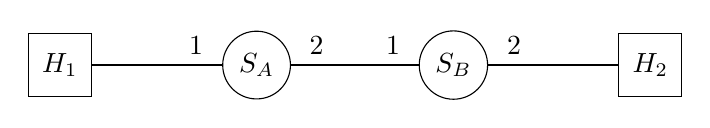
\begin{tikzpicture}[
            node distance={25mm},
            sw/.style = {draw, circle,minimum size=8mm},
            h/.style = {draw, rectangle,minimum size=8mm}
        ]
        \node[h] (h1)  {$H_1$};
        \node[sw] (sa) [right of=h1]  {$S_A$};
        \node[sw] (sb) [right of=sa] {$S_B$};
        \node[h] (h2)  [right of=sb] {$H_2$};
        \draw [thick] (h1)  -- node[above,pos=0.8]{1} (sa);
        \draw [thick] (sa) -- node[above,pos=0.2]{2}
        node[above,pos=0.8]{1}(sb);
        \draw [thick] (sb) -- node[above,pos=0.2]{2} (h2);
    \end{tikzpicture}
    \caption{مثال شبکه}
    \label{netkat:ssh}
\end{figure}
در شکل
\ref{netkat:ssh}
این شبکه شامل دو سوییچ
A و ‌B
و دو هاست می‌باشد.
هر سوییچ دو پورت دارد که با شماره‌های ۱ و۲ مشخص شده‌اند.
در این شبکه هدف این است که امکان جا‌به‌جایی همه‌ی بسته‌ها به غیر از بسته‌هایی که از نوع
SSH
هستند وجود داشته باشد.
عبارت نت‌کت زیر را در نظر بگیرید:
\begin{align*}
    p \triangleq (dst = H_1 \cdot pt \la 1) +
    (dst = H_2 \cdot pt \la 2)
\end{align*}
این عبارت همه‌ی بسته‌هایی که مقصد آن‌ها هاست ۱ باشد را به پورت ۱ و همه‌ی بسته‌هایی که مقصد‌ آن‌ها هاست ۲ باشد را به پورت شماره‌ی ۲ می‌فرستد.
این سیاست به سادگی رفتار سوییچ‌ها را در نت‌کت تعریف می‌کند.
در ادامه می‌توان با اضافه کردن یک فیلتر به این عبارت، دسترسی کنترل را به این سیاست اضافه کرد تا همه‌ی بسته‌های از نوع
SSH
رها شوند:
\begin{align*}
    p_{AC} \triangleq \neg(typ = SSH)\cdot p
\end{align*}
اما استفاده از عبارت بالا به تنهایی برای توصیف رفتار شبکه شکل
\ref{netkat:ssh}
کافی‌ نیست.
برای تکمیل این عبارت لازم است تا رفتار توپولوژی شبکه‌ هم به آن افزوده شود.
در نت‌کت توپولوژی شبکه به عنوان یک گراف جهت‌دار در نظر گرفته می‌شود و رفتار آن در قالب اجتماع رفتار هر یک از لینک‌های آن توصیف می‌شود.
برای شبکه‌ی شکل
\ref{netkat:ssh}
می‌توان از عبارت زیر برای توصیف توپولوژی شبکه استفاده کرد:
\begin{align*}
    t \triangleq & (sw = A \cdot pt = 2 \cdot sw \la B \cdot pt \la 1) +
                 & (sw = b \cdot pt = 1 \cdot sw \la A \cdot pt \la 2) +
                 & (sw = b \cdot pt = 2)
\end{align*}
در نت‌کت در صورتی که سیاست و توپولوژی شبکه در قالب عبارت‌هایی توصیف شده‌باشند،
رفتار کل شبکه در واقع دنباله‌ای از اعمال این عبارت‌ها به صورت یکی در میان است.
به عنوان مثال در شکل
\ref{netkat:ssh}
یک بسته از هاست ۱ ابتدا توسط سوییچ
A
پردازش شده، سپس روی لینک بین دو سوییچ جا به جا می‌شود و در نهایت توسط سوییچ
B
پردازش می‌شود.
در نت‌کت می‌توان این رفتار را به صورت
$p_{AC}\cdot t \cdot p_{AC}$
توصیف کرد.
با استفاده از همین شهود، رفتار کل شبکه را می‌توان در قالب عبارت زیر توصیف کرد:
\begin{align*}
    (p_{AC}\cdot t)^*
\end{align*}
در توصیف بالا فرض شده است که بسته‌ها می‌توانند به هر طریق ممکن وارد شبکه و از آن خارج شوند، اما این رفتار همیشه مورد قبول نیست.
به عنوان مثال در شبکه شکل
\ref{netkat:ssh}
می‌توانیم مکان‌های ورودی یا خروجی شبکه را در قالب عبارت زیر توصیف کنیم:
\begin{align*}
    p_{net} \triangleq e \cdot (p_{AC}\cdot t)^* e
\end{align*}
در حالت کلی‌تر، نیازی به توصیف ورودی و خروجی‌های شبکه در قالب یک عبارت نیست.
پس اگر فرض شود که مکان‌های ورودی شبکه توسط عبارت
$in$
و مکان‌های خروجی شبکه در قالب عبارت
$out$
توصیف شده‌ باشند، رفتار یک شبکه در نت‌کت به صورت زیر تعریف می‌شود:
\begin{align*}
    in \cdot (p\cdot t)^*\cdot out
\end{align*}
که عبارت
$p$
سیاست شبکه و عبارت
$t$
توپولوژی شبکه است.

درستی‌سنجی یک شبکه و بررسی خواص آن در نت‌کت با استفاده از بررسی تساوی عبارت یک شبکه با عبارت‌های دیگر انجام می‌شود.
به عنوان مثال در شبکه‌ی شکل
\ref{netkat:ssh}
برای بررسی اینکه همه‌ی بسته‌ها با نوع
SSH
از هاست ۱ رها می‌شوند کافی است تا تساوی زیر را بررسی کنیم:
\begin{equation}
    \begin{pmatrix}
          type = SSH \cdot sw = A \cdot pt = 1 \cdot \\
          (p_{AC}\cdot t) ^ * \cdot                  \\
          sw = B\cdot pt = 2
    \end{pmatrix}
    \equiv 0
\end{equation}
از طرفی برای بررسی یک خاصیت در شبکه، مثلا امکان فرستاده شدن‌ همه‌ی بسته‌هایی که از نوع
SSH
نیستند از هاست ۱ به هاست ۲
می‌توان به جای بررسی تساوی دو عبارت از نامساوی 
$p \leq q$
استفاده کرد. 
این نامساوی که خلاصه شده‌ی تساوی
$p + q \equiv q$
است بیان می‌کند که رفتار عبارت
$p$
بخشی از رفتار عبارت
$q$
است.
بنابراین برای بررسی این مساله که شبکه‌ی شکل
\ref{netkat:ssh}
به درستی کار می‌کند و فقط بسته‌های 
SSH
را رها می‌کند می‌توان نامساوی زیر را بررسی کرد:
\begin{equation}
    \begin{pmatrix}
          \neg(type = SSH) \cdot sw = A \cdot pt = 1 \cdot &\\
          sw \la B \cdot pt \la 2 &
    \end{pmatrix}
    \leq (p_{AC}\cdot t)^ *
\end{equation}

\section{DyNetKAT}
نک‌کت‌ پویا برای رفع برخی از کاستی‌های نت‌کت ارائه شده است
\cite{dynetkat}.
به صورت دقیق‌تر نت‌کت پویا، امکان توصیف به‌روز‌رسانی سیاست‌های شبکه و همچنین رفتار شبکه در مقابل چندین بسته را ممکن می‌سازد.

\subsection{سینتکس DyNetKAT}
در نت‌کت‌پویا، از رفتار انتها به انتها‌ی توصیف‌های شبکه در قالب عبارت‌های نت‌کت استفاده می‌شود.
به همین منظور سینتکس نت‌کت‌ پویا به صورت زیر تعریف می‌شود:
\begin{align*}
    N & :: = \mathrm{NetKAT}^{-dup}                    \\
    D & :: = \bot | N;D | x?N;D | x!N;D | D\parallel D
    D \oplus D | X                                     \\
      & X \triangleq D
\end{align*}
در سینتکس بالا
$\mathrm{NetKAT}^{-dup}$
قسمتی از زبان نت‌کت است که عبارت‌های
$dup$
از آن حذف شده است.
عبارت‌های
$dup$
در توصیف‌های نت‌کت تاثیری در رفتار یک عبارت ندارند و هدف از استفاده از آن‌ها ثبت یک اثر از هر بسته پس از پردازش توسط یکی از عناصر شبکه است و امکان استدلال بر روی رفتار شبکه را ممکن می‌سازد.
با توجه به این که در نت‌کت پویا رفتار انتها به انتهای یک عبارت نت‌کت مورد استفاده است، عبارت
$dup$
از سینتکس این زبان کنار گذاشته شده است.
نت‌کت‌پویا یک لیست از بسته‌های ورودی را پردازش می‌کند و یک لیست از مجموعه‌ی بسته‌های خروجی را تولید می‌کند.
اپراتور ترکیب متوالی
$N;D$
باعث می‌شود که یک بسته از لیست بسته‌های ورودی توسط سیاست
$N$
پردازش شود و سپس بسته‌ی توسط عبارت
$D$
پردازش می‌شود.
در نت‌کت پویا امکان ارتباط توسط عبارت‌هایی به شکل
$x!N$
و
$x?N$
توصیف می‌شوند که به ترتیب ارسال و دریافت یک عبارت نت‌کت را روی کانال
$x$
توصیف می‌کنند.
ترکیب موازی دو عبارت توسط
$D \parallel D$
توصیف می‌شود.
در نهایت رفتار‌های غیرقطعی توسط‌ عبارت‌هایی به شکل
$D \oplus D$
توصیف می‌شوند.

معنای عملیاتی نت‌کت پویا با استفاده از عبارت‌هایی به شکل
$(d,H,H')$
تعریف می‌شوند که
$d$
عبارت نت‌کت‌ پویا فعلی است،
$H$
لیست بسته‌هایی که در ادامه باید پردازش شوند
و
$H'$
لیست بسته‌هایی است که به صورت موفقیت‌آمیز توسط شبکه پردازش شده‌اند.
برچسب هر قانون که با
$\gamma$
مشخص می‌شود به صورت یکی از شکل‌های
$(\sigma,\sigma'),x!q,x?q$
یا
$rcfg(x,q)$
تعریف می‌شود.
\begin{align}
     & (cpol^{\checkmark}_{\_;})
    \frac{\sigma' \in \sem{p}(\sigma::\his{})}
    {(p;q,\sigma::H,H')\xrightarrow{(\sigma,\sigma')}
    (q,H,\sigma'::H') }                                     \\
     & (cpol_X)
    \frac{(p,H_0,H_1)\xrightarrow{\gamma}(p',H_0',H_1')}
    {(X,H_0,H_1)\xrightarrow{\gamma}(p',H_0',H_1')}
    X \triangleq p                                          \\
     & (cpol_{\_\oplus})
    \frac{(p,H_0,H_0')\xrightarrow{\gamma}(p',H_1,H_1')}
    {(p\oplus q,H_0,H_0')\xrightarrow{\gamma}(p',H_1,H_1')} \\
     & (cpol_{\oplus\_})
    \frac{(q,H_0,H_0')\xrightarrow{\gamma}(q',H_1,H_1')}
    {(p\oplus q,H_0,H_0')\xrightarrow{\gamma}(p',H_1,H_1')} \\
     & (cpol_{\_\parallel})
    \frac{(p,H_0,H_0')\xrightarrow{\gamma}(p',H_1,H_1')}
    {(p\parallel q,H_0,H_0')\xrightarrow{\gamma}(p' \parallel q,H_1,H_1')}
    \\
     & (cpol_{\parallel\_})
    \frac{(q,H_0,H_0')\xrightarrow{\gamma}(q',H_1,H_1')}
    {(p\parallel q,H_0,H_0')\xrightarrow{\gamma}(p \parallel q',H_1,H_1')}
    \\
     & (cpol_?)
    \frac{}
    {(x?p;q,H,H')\xrightarrow{x?p}(q,H,H')}
    \\
     & (cpol_!)
    \frac{}
    {(x!p;q,H,H')\xrightarrow{x!p}(q,H,H')}
    \\
     & (cpol_{!?})
    \frac{
        (q,H,H') \xrightarrow{x!p}(q',H,H')
        (s,H,H') \xrightarrow{x?p} (s',H,H')
    }{
        (q\parallel,H,H') \xrightarrow{rcfg(x,p)} (q'\parallel s',H,H')
    }                                                       \\
     & (cpol_{?!})
    \frac{
        (q,H,H') \xrightarrow{x?p}(q',H,H')
        (s,H,H') \xrightarrow{x!p} (s',H,H')
    }{
        (q\parallel,H,H') \xrightarrow{rcfg(x,p)} (q'\parallel s',H,H')
    }
\end{align}

\begin{figure}
    \centering
    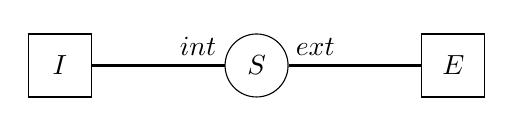
\begin{tikzpicture}[
            node distance={25mm},
            sw/.style = {draw, circle,minimum size=8mm},
            h/.style = {draw, rectangle,minimum size=8mm}
        ]
        \node[h] (i)  {$I$};
        \node[sw] (s) [right of=i]  {$S$};
        \node[h] (e)  [right of=s] {$E$};
        \draw [thick] (i)  -- node[above,pos=0.8]{$int$} (s);
        \draw [thick] (s) -- node[above,pos=0.2]{$ext$} (e);
    \end{tikzpicture}
    \caption{مثال دیوار آتش}
    \label{dynetkat:firewall}
\end{figure}

در ادامه چگونگی توصیف مثال دیوار آتش در شکل
\ref{dynetkat:firewall}
بیان می‌شود.
در این شبکه هدف این است که امکان ارتباط از داخل شبکه فراهم باشد ولی امکان ارسال بسته از خارج شبکه ممکن نباشد.
اما زمانی که یک بسته به خارج ارصال شد، دیوار آتش اجازه‌ی عبور بسته‌ها از بیرون را می‌دهد تا پاسخ بسته‌ها داده شود.
برای توصیف این شبکه می‌توان از عبارت نت‌کت پویای زیر استفاده کرد:
\begin{align*}
    Host  \triangleq   & secConReq!1;Host \oplus secConEnd!1;Host        \\
    Switch \triangleq  & (port = int) \cdot (port \la ext);Switch \oplus \\
                       & (port = ext)\cdot 0 ; Switch \oplus             \\
                       & secConReq?1;Switch'                             \\
    Switch' \triangleq & (port =int) \cdot (port \la ext);Switch' \oplus \\
                       & (port=ext)\cdot(port\la int);Switch' \oplus     \\
                       & secConEnd?1;Switch                              \\
    Init \triangleq    & Host \parallel Switch
\end{align*}
در این توصیف هاست امکان ارسال پیام برای شروع یا خاتمه‌ی یک ارتباط امن را دارد.
رفتار سوییچ در ابتدا به این صورت تعریف شده است که بسته‌ها را از پورت داخلی به پورت خارجی ارسال کند و تمام بسته‌هایی که از پورت خروجی وارد می‌شوند رها کند.
همچنین سوییچ امکان دریافت پیام شروع ارتباط امن را دارد.
پس از دریافت این پیام سوییچ اجازه می‌دهد تا بسته‌ها از پورت خروجی وارد شبکه شوند.
همچنین در صورتی که پیام خاتمه‌ی ارتباط امن را دریافت کند دوباره به رفتار اولیه‌ی خود بر می‌گردد.
در نهایت رفتار کل شبکه با استفاده از ترکیب موازی یک هاست و یک سوییچ در حالت اولیه توصیف می‌شود.
\begin{figure}[ht]
    \centerline{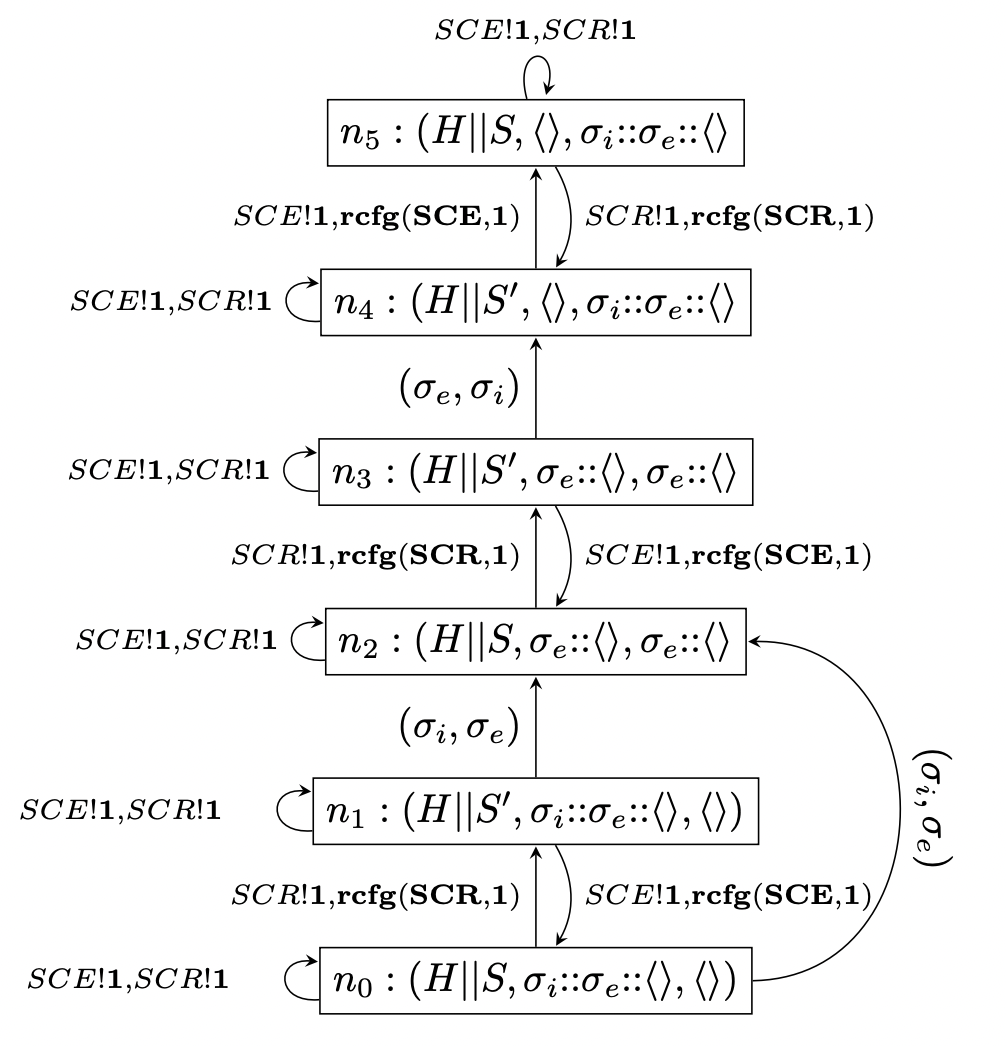
\includegraphics[width=0.8\textwidth]{mine/firewall-lts.png}}
    \caption{سیستم انتقال برچسب‌دار برای شبکه‌ی دیوار آتش}
    \label{firewall:lts}
\end{figure}
نمودار نمایش داده شده در شکل
\ref{firewall:lts}
سیستم انتقال این شبکه‌ را در حالتی که یک بسته روی پورت ورودی و یک بسته روی پورت خروجی شبکه وجود دارد نشان می‌دهد.
همانطور که در نمودار مشخص است، عملیات 
$(\sigma_e,\sigma_i)$
که به معنای ارسال بسته از پورت ورودی به پورت خروجی است تنها در قسمتی از این سیستم انتقال قابل دسترسی است که پیش از آن یکی از عملیات‌های 
$SCR?1$
یا
$rcfg(SCR,1)$
انجام شده باشند.
بنابراین در این حالت شبکه تنها در صورتی که بسته خارجی را به داخل ارسال می‌کند که پیش از آن پیام آغاز ارتباط امن دریافت کرده‌ باشد.


